\documentclass[12pt, a4paper]{article}
\usepackage[margin=0.7in]{geometry}
\usepackage{tikz}
\usetikzlibrary{positioning, shapes.geometric, arrows.meta, fit, backgrounds, matrix}
\usepackage{xcolor}
\usepackage{graphicx}
\usepackage{hyperref}
\hypersetup{
    colorlinks=true,
    linkcolor=blue,
    filecolor=magenta,      
    urlcolor=cyan,
}

\title{AI Music Recommender System \\ Architecture \& User Flow Diagram}
\author{Deployed with Docker Compose}
\date{\today}

\begin{document}

\maketitle

\begin{abstract}
    This document presents a comprehensive architectural diagram of a containerized AI Music Recommender System. The system employs a microservices architecture orchestrated by Docker Compose, featuring a React.js frontend, Flask backend with machine learning recommendation engine, and multiple data stores (PostgreSQL, Redis, Qdrant). The diagram visualizes user interactions, API call flows, database queries, and inter-service communication across the deployed containers.
\end{abstract}

\section*{Architecture Summary}
The system is designed as a three-tier application:
\begin{itemize}
    \item \textbf{Presentation Layer (Green):} User-facing components including browser, NGINX reverse proxy, and React.js SPA.
    \item \textbf{Application Layer (Orange):} Business logic and AI components with Flask backend and Recommendation Engine.
    \item \textbf{Data Layer (Purple):} Persistent and ephemeral storage systems for user data, music metadata, and vector embeddings.
\end{itemize}

All services are containerized and managed via Docker Compose, ensuring environment consistency, simplified deployment, and service isolation. Communication follows RESTful API patterns between frontend/backend and dedicated protocols for database interactions.

\clearpage

\section*{System Architecture Diagram}

\begin{center}
\begin{tikzpicture}[
    >=Stealth,
    node distance=0.7cm and 1cm,
    service/.style={rounded rectangle, draw=black, thick, align=center, minimum width=3cm, minimum height=1.5cm, font=\small},
    db/.style={cylinder, shape border rotate=90, draw=black, thick, aspect=0.3, align=center, minimum height=1.8cm, font=\small},
    group/.style={rectangle, rounded corners, inner sep=10pt},
    legendbox/.style={rectangle, draw=black, thin, align=left, anchor=north west, font=\scriptsize},
    apiarrow/.style={->, thick, blue!70!black},
    dbarrow/.style={->, dashed, thick, violet!70!black},
    userflow/.style={->, thick, green!50!black},
    label/.style={font=\tiny\itshape, align=center},
    mymatrix/.style={matrix of nodes, nodes={rectangle}, row sep=0.2cm, column sep=0.5cm}
]

% ==================== USER LAYER ====================
\node[service, fill=green!20] (browser) {\textbf{User Browser}\\(Chrome/Firefox/Safari)};

% ==================== FRONTEND LAYER (GREEN) ====================
\node[service, fill=green!20, right=2.8cm of browser] (nginx) {\textbf{NGINX}\\\scriptsize Reverse Proxy\\Ports 80/443};
\node[service, fill=green!20, right=2.8cm of nginx] (frontend) {\textbf{React.js}\\\scriptsize Frontend\\Port 3000};

% Layer labels
\node[above=0.05cm of browser, font=\bfseries\tiny, align=center] (userlabel) {Client Layer};
\node[above=0.05cm of nginx, font=\bfseries\tiny, align=center] (frontendlabel) {Frontend Layer};

% User to Frontend flow
\draw[userflow] (browser.east) -- node[above, sloped, label] {HTTPS/HTTP} (nginx.west);
\draw[apiarrow] (nginx.east) -- node[above, sloped, label] {Static Assets\\Proxy Pass} (frontend.west);

% Frontend group background
\begin{scope}[on background layer]
    \node[group, fill=green!10, draw=green!40, thick, fit=(browser) (nginx) (frontend) (userlabel) (frontendlabel)] (frontendgroup) {};
\end{scope}

% ==================== BACKEND LAYER (ORANGE) ====================
\node[service, fill=orange!20, below=2.5cm of nginx] (backend) {\textbf{Flask Backend}\\\scriptsize REST API\\Port 5000};
\node[service, fill=orange!20, right=1.8cm of backend] (engine) {\textbf{Recommendation}\\\textbf{Engine}\\\scriptsize AI/ML Model};

% Backend layer label
\node[above=0.05cm of backend, font=\bfseries\tiny, align=center] (backlabel) {Backend Layer};

% Backend group background
\begin{scope}[on background layer]
    \node[group, fill=orange!10, draw=orange!40, thick, fit=(backend) (engine) (backlabel)] (backendgroup) {};
\end{scope}

% Frontend to Backend API calls
\draw[apiarrow] (frontend.south) .. controls +(down:1.5cm) and +(up:1cm) ..
    node[right, pos=0.6, label, align=left, xshift=0.3cm] {API Calls:\\• Login/Register\\• Get Recommendations\\• Set Mood\\• Quick Mix} (backend.north);

% Backend internal communication
\draw[apiarrow, <->] (backend.east) -- node[above, label, yshift=0.1cm] {Model Inference} (engine.west);

% ==================== DATA LAYER (PURPLE) ====================
\node[db, fill=purple!20, below=1.8cm of backend] (postgres) {\textbf{PostgreSQL}\\Port 5432\\\tiny Users, Tracks,\\Mood Prefs};
\node[db, fill=purple!20, left=1.8cm of postgres] (redis) {\textbf{Redis}\\Port 6379\\\tiny Session Cache};
\node[db, fill=purple!20, right=1.8cm of postgres] (qdrant) {\textbf{Qdrant}\\Port 6333\\\tiny Vector DB\\Music Embeddings};

% Data layer label
\node[above=0.05cm of postgres, font=\bfseries\tiny, align=center] (datalabel) {Data Layer};

% Data group background
\begin{scope}[on background layer]
    \node[group, fill=purple!10, draw=purple!40, thick, fit=(postgres) (redis) (qdrant) (datalabel)] (datagroup) {};
\end{scope}

% Backend to Data connections
\draw[dbarrow] (backend.south) -- node[left, pos=0.5, label, xshift=-0.2cm] {User Queries\\CRUD Ops} (postgres.north);
\draw[dbarrow] (backend.south west) .. controls +(left:0.6cm) and +(up:0.4cm) ..
    node[above, sloped, label] {Cache\\Read/Write} (redis.north east);
\draw[dbarrow] (engine.south) .. controls +(down:0.6cm) and +(up:0.4cm) ..
    node[above, sloped, label] {Similarity\\Search} (qdrant.north west);
\draw[dbarrow] (backend.south east) .. controls +(right:0.2cm) and +(west:0.4cm) ..
    node[below, sloped, label, yshift=-0.1cm] {Metadata\\Lookup} (qdrant.west);

% ==================== DOCKER COMPOSE VISUALIZATION ====================
\node[below=1.2cm of datagroup.south, font=\bfseries\small, align=center] (dockerlabel) {Docker Compose Orchestration};

% Docker container box
\node[service, fill=white, draw=gray, thick, below=0.4cm of dockerlabel, 
      minimum width=14cm, minimum height=0.8cm, align=center, font=\small] (docker) 
      {\texttt{docker-compose.yml} (Orchestrates all services)};

% Connecting services to docker box
\foreach \source in {frontend, backend, postgres, redis, qdrant}
    \draw[gray, thick, dotted, looseness=1.2] (\source.south) .. controls +(down:1.2cm) and +(north:0.6cm) .. (docker.north);

% ==================== MAIN DIAGRAM BOUNDING BOX ====================
\begin{scope}[on background layer]
    \node[draw=black!20, dashed, thick, inner sep=15pt, fit=(frontendgroup) (backendgroup) (datagroup) (docker) (dockerlabel)] (mainbox) {};
\end{scope}

\end{tikzpicture}

% ==================== SEPARATE LEGENDS (outside tikzpicture for better positioning) ====================
\vspace{1.5cm}

\begin{center}
\begin{tikzpicture}[
    legendbox/.style={rectangle, draw=black, thin, align=left, font=\scriptsize, inner sep=8pt},
    legendtitle/.style={font=\bfseries\small, align=center}
]

% Flow Legend on the left
\node[legendbox, text width=6.5cm, anchor=north west] at (0,0) {
    \textbf{Flow Legend:}\\[0.2cm]
    \begin{tikzpicture}[scale=0.65, transform shape]
        \draw[->, thick, blue!70!black] (0,0) -- (3,0) node[right, font=\tiny] {REST API Calls};
        \draw[->, dashed, thick, violet!70!black] (0,-0.5) -- (3,-0.5) node[right, font=\tiny] {Database Queries};
        \draw[->, thick, green!50!black] (0,-1) -- (3,-1) node[right, font=\tiny] {User Requests};
        \draw[gray, thick, dotted] (0,-1.5) -- (3,-1.5) node[right, font=\tiny] {Docker Network};
    \end{tikzpicture}\\[0.3cm]
    \textbf{Key Interactions:}
    \begin{itemize}
        \setlength\itemsep{0em}
        \item[\textcolor{blue}{\textbullet}] \textbf{Login:} Auth flow with Redis session
        \item[\textcolor{blue}{\textbullet}] \textbf{Mood Selection:} Updates user preferences in PostgreSQL
        \item[\textcolor{blue}{\textbullet}] \textbf{Recommendations:} Vector search in Qdrant + filtering
        \item[\textcolor{blue}{\textbullet}] \textbf{Quick Mix:} Cached playlist generation
    \end{itemize}
};

% Docker Services Legend on the right
\node[legendbox, text width=7.5cm, anchor=north west] at (7.5,0) {
    \textbf{Docker Services Legend:}\\[0.1cm]
    \begin{tabular}{|p{2.3cm}|p{3.2cm}|p{1.3cm}|}
        \hline
        \textbf{Service} & \textbf{Image/Container} & \textbf{Port} \\
        \hline
        Reverse Proxy & nginx:alpine & 80:80 \\ & & 443:443 \\
        \hline
        Frontend & node:18-alpine + react-app & 3000:3000 \\
        \hline
        Backend API & python:3.11-slim + flask & 5000:5000 \\
        \hline
        Database & postgres:15-alpine & 5432:5432 \\
        \hline
        Cache & redis:7-alpine & 6379:6379 \\
        \hline
        Vector DB & qdrant/qdrant & 6333:6333 \\
        \hline
    \end{tabular}\\[0.3cm]
    \textbf{Data Persistence:}
    \begin{itemize}
        \setlength\itemsep{0em}
        \item PostgreSQL: \texttt{postgres\_data}
        \item Redis: \texttt{redis\_data}
        \item Qdrant: \texttt{qdrant\_storage}
        \item NGINX SSL: \texttt{nginx\_certs}
    \end{itemize}
};

\end{tikzpicture}
\end{center}

% ==================== ARCHITECTURE NOTES ====================
\vspace{0.8cm}
\begin{center}
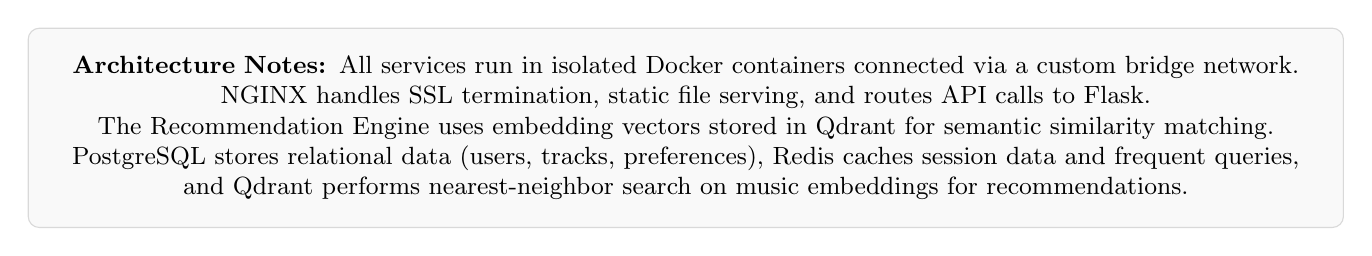
\begin{tikzpicture}
\node[draw=gray!30, fill=gray!5, rounded corners, inner sep=10pt, text width=16cm, align=center, font=\small] {
    \textbf{Architecture Notes:} All services run in isolated Docker containers connected via a custom bridge network. \\
    NGINX handles SSL termination, static file serving, and routes API calls to Flask. \\
    The Recommendation Engine uses embedding vectors stored in Qdrant for semantic similarity matching. \\
    PostgreSQL stores relational data (users, tracks, preferences), Redis caches session data and frequent queries, \\
    and Qdrant performs nearest-neighbor search on music embeddings for recommendations.
};
\end{tikzpicture}
\end{center}

\end{document}

\clearpage

\section*{Deployment \& Execution Instructions}
\subsection*{Prerequisites}
\begin{itemize}
    \item Docker Engine 20.10+ and Docker Compose v2.0+
    \item Git for version control
    \item Minimum 4GB RAM, 2 CPU cores, 10GB disk space
\end{itemize}

\subsection*{Quick Start}
\begin{verbatim}
# Clone repository
git clone https://github.com/example/ai-music-recommender
cd ai-music-recommender

# Configure environment variables
cp .env.example .env
# Edit .env with your settings

# Build and start all services
docker-compose up --build -d

# View logs
docker-compose logs -f

# Access application
# Frontend: https://localhost (or http://localhost:80)
# Backend API: http://localhost:5000/api
\end{verbatim}

\subsection*{Service Health Checks}
\begin{verbatim}
# Check container status
docker-compose ps

# Test backend API
curl http://localhost:5000/api/health

# Test database connections
docker exec -it music_postgres pg_isready
docker exec -it music_redis redis-cli ping
\end{verbatim}

\subsection*{Data Persistence}
Docker volumes are configured for:
\begin{itemize}
    \item PostgreSQL data: \texttt{postgres\_data}
    \item Redis data: \texttt{redis\_data}
    \item Qdrant storage: \texttt{qdrant\_storage}
    \item NGINX SSL certificates: \texttt{nginx\_certs}
\end{itemize}

\subsection*{Scaling Considerations}
\begin{itemize}
    \item Frontend: Scale horizontally behind NGINX load balancer
    \item Backend: Use multiple Flask workers (Gunicorn) or container replicas
    \item Redis: Implement Redis Cluster for high availability
    \item Qdrant: Deploy in cluster mode for larger embedding datasets
\end{itemize}

\section*{Troubleshooting}
\begin{itemize}
    \item \textbf{Port conflicts:} Modify ports in \texttt{docker-compose.yml} and \texttt{.env}
    \item \textbf{High memory usage:} Limit container memory in compose file
    \item \textbf{SSL errors:} Ensure certificates are mounted correctly in NGINX
    \item \textbf{Database connection failures:} Check network connectivity between containers
\end{itemize}

\end{document}